\documentclass[russian, hyperref={unicode}]{beamer}

\usetheme{Madrid}
\setbeamertemplate{footline}[frame number]
\setbeamertemplate{navigation symbols}{}
\setbeamerfont{note page}{size=\footnotesize}
\setbeamertemplate{note page} {%
  \hbox{\insertshortframetitle[width=8cm]}%
  \vskip1.75em
  \nointerlineskip
  \insertnote
}

% \setbeameroption{show only notes}

\usepackage[T2A]{fontenc}
\usepackage{lmodern}
\usepackage[utf8x]{inputenc}
\usepackage[english, russian, main=russian]{babel}
\usepackage{graphicx}
\usepackage{tikz}

\usepackage{algpseudocode}
\algtext*{EndWhile}     % Remove "end while" text
\algtext*{EndFor}       % Remove "end for" text
\algtext*{EndFunction}  % Remove "end function" text
\algtext*{EndIf}        % Remove "end if" text

\graphicspath{ {../Images/} }

\newcommand{\inputTikZ}[1]{\input{../Images/#1.tikz}}

% workaround warning
\let\Tiny=\tiny

\title{Разработка алгоритмов статического поиска выходов за пределы
  динамического массива в С/C++ программах}
\author{И. Е. Громаковский \\
  {\small Научный руководитель: М. А. Лукин}}
\institute{Санкт-Петербургский национальный исследовательский
  университет \\ информационных технологий, механики и оптики}
\date{}

\begin{document}

\section{Введение}

\frame{\titlepage}
\note{Здравствуйте!}

\subsection{Решаемая проблема}

\begin{frame}{Описание задачи}
    \begin{itemize}
        \item Статический поиск выходов за пределы динамического
          массива в C и C++.
        \item Работа с большими программами за разумное время.
        \item В общем случае задача поиска всех выходов неразрешима.
        \item Находить как можно больше ошибок, минимизируя число
          ложных срабатываний.
    \end{itemize}
\end{frame}
\note {
  Как видно из названия, в рамках данной работы требуется находить
  выходы за пределы динамического массива в программах на C и
  C++. Делать это нужно статически, что позволяет найти ошибки до
  того, как они проявят себя. Требуется уметь обрабатывать большие
  программы (состоящие из сотен тысяч строк) за разумное время. В
  общем случае задача поиска всех выходов за пределы массива
  неразрешима, поэтому неформально задача состоит в поиске как можно
  большего числа ошибок с максимальной точностью.
}

\begin{frame}{Актуальность проблемы}
    \begin{itemize}
        \item Программное обеспечение всегда было и остаётся
          подвержено ошибкам в коде.
        \item Выход за пределы массива — одна из главных уязвимостей с
          точки зрения безопасности.
        \item Особенно опасны ошибки в операционных системах, для
          которых популярны языки C и C++.
    \end{itemize}
\end{frame}
\note {
  Данная проблема является крайне актуальной, поскольку программное
  обеспечение всегда было и остаётся подвержено ошибкам в
  коде. Известно большое число примеров, когда ошибки в коде
  приводили к ужасным последствиям. Ошибки, ведущие к выходу за
  пределы массива в C/C++, являются одной из главных уязвимостей с
  точки зрения безопасности. В некоторых случаях злоумышленник может,
  используя такие уязвимости, получить полный контроль над
  системой. Стоит отметить, что особую опасность представляют такие
  ошибки в коде операционных систем, виртуальных машин и прочих
  низкоуровневых программ. Они зачастую пишутся на C/C++, что
  усиливает актуальность проблемы.
}

% \subsection{Обзор существующих решений}

% \begin{frame}{Существующие решения}
%     \begin{itemize}
%         \item Использование аннотаций (Dor et al., 2003)
%         \item Вывод ограничений
%           \begin{itemize}
%             \item Обход путей программы, построение логического
%               утверждения (Ganapathy et al., 2003)
%             \item Анализ по требованию (Le et al., 2008)
%           \end{itemize}
%         \item Анализ промежуточного представления (Li et al., 2010)
%     \end{itemize}
% \end{frame}
% \note {
%   \tiny
%   Среди существующих решений можно выделить некоторые общие
%   подходы. Например, некоторые подходы используют пользовательские
%   аннотации для упрощения проверки корректности доступа к
%   памяти. Однако для больших программ такой подход требует слишком
%   больших человеческих усилий для написания аннотаций, поэтому он
%   практически не применим. Большинство известных подходов выводят
%   ограничения различных значений в программе и делают вывод о наличии
%   ошибок, исходя из этих ограничений. Один из вариантов заключается в
%   обходе всех путей программы и построении системы, ограничивающей
%   возможные значения переменных, а также логического утверждения,
%   соответствующего отсутствию ошибок. После этого используется
%   SMT-solver для проверки выполнимости этого утверждения. При большом
%   числе ветвлений такой подход работает неприемлемо. Более новой
%   является идея анализа по требованию, суть которого
%   состоит в том, чтобы рассматривать только пути программы, которые
%   влияют на обращения к массиву. Вместо описания программы в целом,
%   каждое обращение обрабатывается отдельно, что на практике
%   существенно уменьшает объём вычислений. Также стоит отметить
%   использование промежуточного представления, например, представление
%   LLVM, для анализа.
% }

\subsection{Основа работы}

\begin{frame}{Анализ LLVM-IR}
\begin{itemize}
  \item Меньше языковых конструкций, проще анализ.
  \item Анализируемый код ближе к реально выполняемому.
  \item Встроенные оптимизации и средства для анализа кода.
  \item Автоматически поддерживается любой язык, для которого есть
    компилятор в LLVM-IR.
  \item Static Single Assignment.
\end{itemize}
\end{frame}
\note {
  Анализ LLVM IR имеет несколько преимуществ. Во-первых, в
  промежуточном представлении меньше языковых конструкций, что
  упрощает анализ. Во-вторых, анализируемый код ближе к реально
  выполняемому, что позволяет учесть влияние компилятора. Также в LLVM
  имеется большое число встроенных оптимизаций и средств для анализа
  кода. Анализатор LLVM IR позволяет анализировать любой язык, для
  которого есть компилятор в LLVM IR, в частности C/C++. Ещё одним
  преимуществом является то, что программа в LLVM IR представлена в
  static single assignment форме, которая крайне удобна для анализа. В
  static single assignment форме значение каждой переменной
  присваивается ровно один раз, а в местах слияния различных значений
  одной переменной используются фи-функции.
}

\begin{frame}{Li, Cifuentes, Keynes: ranges}
  \begin{itemize}
    \item Li L., Cifuentes C., Keynes N. Practical and Effective
      Symbolic Analysis for Buffer Overflow Detection.
    \item Symbolic ranges.
      \begin{itemize}
        \item Symbolic expressions: $15$, $x + 1$, $\bot$, $\top$.
        \item Частичный порядок.
        \item Symbolic range: $[s1, s2]$.
        \item Операции: $\cup, \cap, +, -, \times, \div$.
      \end{itemize}
    \item Define range, $S_v$:
      \begin{itemize}
        \item в месте определения $V$.
      \end{itemize}
    \item Use range, $S_{V, P}$:
      \begin{itemize}
        \item в произвольном месте $P$.
      \end{itemize}
    \item Выход за пределы массива размера $n$:
      \begin{itemize}
        \item $S_{n, P}^{max} \prec S_{index, P}^{max} \vee S_{index,
            P}^{min} \prec -1$.
      \end{itemize}
  \end{itemize}
\end{frame}
\note {
  В основе данной работы лежит работа Li, Cifuentes, Keynes. Я
  вкратце расскажу суть. В их работе вводится понятие symbolic
  range. Сначала определяется symbolic expression, которым может быть
  константа, переменная, аффиная функция от других symbolic
  expressions, а также bot and top, соответствующие минимальному и
  максимальному значению. На symbolic expressions естественным образом
  задаётся частичный порядок. Symbolic range — пара из symbolic
  expressions. Для symbolic range вводятся операции объединения,
  пересечения, сложения, вычитания, умножения, деления.  Для каждой
  переменной вводится понятие define range — диапазон её значений в
  месте определения.  Также вводится понятие use range — диапазон
  значений переменной в произвольной точке программы. Этот диапазон
  может быть меньше define range, т. к. в некоторые инструкции в
  программе можно прийти только по условным переходам. Например, если
  инструкция под $if (x < 0)$, то в ней $x$ точно меньше нуля.
  Анализатор сообщает о выходе за пределы массива, если максимально
  возможное значение размера может быть меньше либо равно значения
  индекса или если индекс может быть отрицательным.
}

\begin{frame}{Li, Cifuentes, Keynes: зависимости}
  \begin{itemize}
    \item Зависимости по данным
      \begin{itemize}
        \item Define range вычисляется через диапазоны аргументов.
        \item $S_{(a + b)} = S_{a, P} + S_{b, P}, P = a + b$
        \item $S_{(\phi(a, b))} = S_{a, P} \cup S_{b, P}, P = \phi(a, b)$
      \end{itemize}
    \item Зависимости потока управления
      \begin{itemize}
        \item Уточнение диапазона $S_{V, P}$ на основании предикатов на пути к $P$.
        \item Предикаты, связанные с $V$, такие что:
          \begin{itemize}
            \item $P$ строго доминируется предикатом;
            \item $P$ достижима только из одного потомка условного перехода.
          \end{itemize}
      \end{itemize}
  \end{itemize}
\end{frame}
\note {
  Для расчёта диапазонов значений рассматриваются два вида
  зависимостей.
  Зависимости по данным используются для вычисления define
  range. Например, define range суммы является суммой use ranges
  аргументов в инструкции сложения. Define range фи-инструкции
  является объединением use ranges, т. к. фи может вернуть любое из значений.
  Зависимости потока управления используются для уточнения диапазона
  значений в инструкции $P$ на основании предикатов на пути к $P$ по
  графу потока управления. Для уточнения диапазона значений $V$
  используются предикаты, затрагивающие $V$, такие что выполнены два
  условия. Дальше по слайду.
}

\section{Улучшения}

\subsection{Обработка циклов}

\begin{frame}{Монотонно изменяющиеся переменные}
    \begin{columns}
        \column{.5\textwidth}
            \begin{figure}
                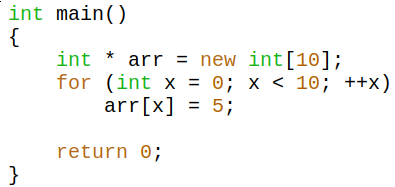
\includegraphics[width=\textwidth, clip=true]{for-trivial.png}
            \end{figure}
        \column{.5\textwidth}
            \begin{figure}
                \inputTikZ{for-trivial}
            \end{figure}
    \end{columns}
    \begin{itemize}
      \item Нет предикатов, ограничивающих значение снизу.
      \item Если $x = \phi(a, b), b = f(x)$ и последовательность $x,
        f(x), f(f(x)) \ldots$ монотонна (например, возрастает), то
        применяется предикат $x \geq a (x \leq a)$.
    \end{itemize}
\end{frame}
\note {
  У описанного в статье подхода есть определённые недостатки,
  которым было уделено внимание в моей работе. Рассмотрим пример на
  слайде. В данном случае нет предиката, ограничивающего значение $x$
  снизу. Алгоритм будет работать следующим образом: поскольку значение
  $x$ зависит от $x_1$, которое в свою очередь зависит от $x$, то
  первоначально в качестве значения $x$ будет взят отрезок
  $[\bot, \top]$. Затем будет учтён предикат, что $x < 10$ в месте
  вычисления $x_1$. В результате диапазон значений $x_1$ будет
  $[\bot, 10]$, диапазон значений $x$ будет такой же. Таким образом
  использование $x$ в качестве индекса будет считаться ошибочным,
  поскольку анализатор посчитает, что он может быть
  отрицательным. Однако нетрудно видеть, что это не так.  Для решения
  этой проблемы вводится правило, описанное на слайде.
}

\begin{frame}{Обработка предиката «не равно»}
    \begin{columns}
        \column{.5\textwidth}
            \begin{figure}
                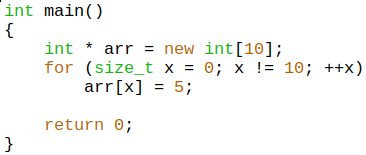
\includegraphics[width=\textwidth, clip=true]{for-ne.png}
            \end{figure}
        \column{.5\textwidth}
            \begin{figure}
                \inputTikZ{for-ne}
            \end{figure}
    \end{columns}
    \begin{itemize}
      \item Алгоритм из статьи учитывает $x != y$, только если значение на
        границе отрезка.
      \item Если $x = \phi(a, f(x)), \exists c: y = f^c(a)$ и
        последовательность $x, f(x), f(f(x)), \ldots$ монотонна
        (например, возрастает), то применяется предикат $x < y$.
    \end{itemize}
\end{frame}
\note {
  Следующее улучшение связано с обработкой условия «не
  равно». Согласно алгоритму из статьи, условие $x \neq y$ учитывается
  только в том случае, если равенство $x = y$ выполняется для
  граничного значения рассматриваемой переменной. Из-за этого алгоритм
  неспособен корректно обрабатывать циклы, в которых значение счётчика
  ограничено таким предикатом, хотя они встречаются в программах
  крайне часто. Например, в простейшем цикле, представленном на
  рисунке, значение переменной $x$ в месте записи в массив не будет
  ограничено, поскольку число $10$ не лежит на границе отрезка
  значений $x$. Для решения этой проблемы вводится следующее
  правило. Если $x$ является $\phi$ функцией от какого-то значения $a$
  и другого значения, представленного функцией от $x$, и существует
  такая константа $c$, что $c$ последовательных применений $f$ к $a$
  возвращают $y$, а также последовательность применений $f$ к
  аргументу монотонна, то применяется предикат $x < y$ (или $x > y$ в
  зависимости от характера монотонности).
}

\begin{frame}{Улучшение учёта предикатов}
    \begin{columns}
        \column{.5\textwidth}
            \begin{figure}
                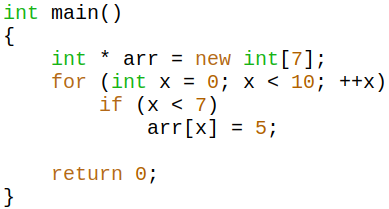
\includegraphics[width=\textwidth, clip=true]{predicates-improvement.png}
            \end{figure}
        \column{.5\textwidth}
            \begin{figure}
                \inputTikZ{predicates-improvement}
            \end{figure}
    \end{columns}
    \begin{itemize}
      \item Запись в массив достижима из обоих потомков условного
        перехода.
      \item Решение: игнорировать рёбра, проходящие через предикат.
    \end{itemize}
\end{frame}
\note {
  Ещё одно улучшение затрагивает правила для учёта
  предикатов. Рассмотрим пример на слайде, здесь значение $x$ внутри
  цикла дополнительно ограничено семью, что делает запись в массив
  корректной. Однако согласно алгоритму из статьи предикат,
  ограничивающий значение $x$, должен быть учтён только в том случае,
  если запись в массив достижима только из одного потомка условного
  перехода. Нетрудно видеть, что в данном случае запись в массив
  достижима из обоих потомков, из-за чего предикат не будет учтён, что
  приведёт к false positive. Для решения проблемы предлагается
  модификация этого правила, состоящая в игнорировании рёбер,
  проходящих через предикат, при проверке наличия путей из потомков.
}

\begin{frame}{Межпроцедурный анализ}
    \begin{itemize}
      \item Функции анализируются в порядке топологической сортировки.
      \item Циклы в графе вызовов анализируются в произвольном порядке.
      \item При вызове функции запоминаются диапазоны аргументов
        (целочисленных переменных и размеров массивов).
      \item При повторном вызове диапазоны объединяются.
    \end{itemize}
\end{frame}
\note {
  Описанный в статье алгоритм рассматривает каждую функцию отдельно,
  не учитывая зависимости между функциями. Последнее улучшение состоит
  в добавлении учёта этих зависимостей. Для этого функции
  анализируются в порядке топологической сортировки, от вызывающей к
  вызываемой. Если в графе вызовов есть цикл, то для него
  топологическая сортировка невозможна, и он анализируется в
  произвольном порядке. При вызове функции в глобальный контекст
  сохраняется диапазон значений каждого аргумента. При повторном
  вызове диапазоны объединяются. Таким образом, при анализе функции
  для её аргументов известны диапазоны возможных значений. Если
  функция ни разу не вызывалась, то считаем, что её аргументы могут
  принимать любые значения.
}

\section{Результаты}

\begin{frame}{Результаты}
  \begin{tabular}{|*{18}{c|}}\hline
  Software         & LOC  & .bc & Time  & Reports & TP & FP \\\hline
  PostgreSQL 8.3.0 & 450k & 26M & 6:28  & 16      & 10 & 6  \\\hline
  CMake 3.1.0      & 350k & 31M & 11:03 & 10      & 5  & 5  \\\hline
  \end{tabular}
\end{frame}
\note {
  На данном слайде показана таблица с результатами применения
  анализатора к крупным open-source проектам. Колонка .bc показывает
  размер байткода, подаваемого на вход анализатору. Хоть CMake
  содержит меньше строк кода, байткод файл получился больше, и анализ
  занял больше времени, поскольку в CMake используется преимущественно
  C++, а не C. Видно, что анализатор работает за разумное время для
  крупных проектов и способен находить ошибки. К сожалению, не
  обошлось без относительно большого числа false positive, однако
  такие показатели весьма приемлимы для легковесного анализатора.
}

\begin{frame}{Сравнение}
  \begin{table}[h]
  \centering
  \begin{tabular}{|*{18}{c|}}\hline
  --             & TP  & FP & FN \\\hline
  Clang Analyzer & 0   & 0  & 0  \\\hline
  CppCheck       & 3   & 0  & 9  \\\hline
  PVS-Studio     & 4   & 0  & 8  \\\hline
  Splint         & 9   & 3  & 3  \\\hline
  Li et at.      & 12  & 8  & 0  \\\hline
  Improved       & 12  & 0  & 0  \\\hline
  \end{tabular}
  \end{table}
\end{frame}
\note {
  Также было произведено сравнение с другими свободно
  распространяемыми анализаторами. Поскольку найти проект, на котором
  представленные анализаторы работают из коробки, не удалось, был
  собран набор различных примеров работы с массивом. Clang Analyzer
  не нашёл ни одной ошибки. CppCheck и PVS-Studio проводят
  межпроцедурный анализ, однако смогли найти лишь 3 и 4 ошибки
  соответственно. Из достоинств стоит отметить отсутствие ложных
  срабатываний. Split, в отличие от предыдущих двух, сообщает об
  ошибках всегда, когда не может доказать обратного. За счёт этого
  удалось найти 9 ошибок, однако так же было 3 ложных срабатывания,
  одно из них — из-за отсутствия межпроцедурного анализа. Также splint
  умеет работать только с C кодом, но не C++. Версия анализатора,
  реализованная в точном соответстии с упомянутой ранее статьёй,
  успешно нашла все 12 ошибок, однако также было 8 ложных срабатываний
  по причинам, описанным выше. Наконец, улучшенная версия также нашла
  все ошибки, но без единого false positive.
}

\begin{frame}{Заключение}
    \begin{itemize}
        \item За основу взят известный подход.
        \item Выявлены недостатки подхода.
        \item Сделаны улучшения, направленные на устранение выявленных
          недостатков.
        \item Получился легковесный анализатор, способный находить
          ошибки в больших программах, работающий лучше доступных анализаторов.
    \end{itemize}
\end{frame}
\note { Таким образом, в рамках данной работы за основу был взят
  известный легковесный подход, были выявлены различные недостатки и
  сделаны улучшения, направленные на устранение этих недостатков. В
  результате получился легковесный анализатор, способный находить
  ошибки в больших программах и работающий лучше доступных
  анализаторов.
}

\begin{frame}{Спасибо за внимание!}
    \begin{center}
        \Huge
        {\color{blue} Вопросы?}
    \end{center}
\end{frame}
\note{До свидания!}

% \appendix

% \begin{frame}[noframenumbering, t]{Обоснование метрик}
%     \only<1> {
%       kek
%     }
%     \only<2> {
%       хи-хи
%     }
% \end{frame}

\end{document}
